% !TEX root = C:/university/year_FS22/et2_labor/sw4/report/main.tex
\documentclass[../main.tex]{subfiles}

\begin{document}
\section{Messschaltung}

\begin{figure}[h]
  \centering
  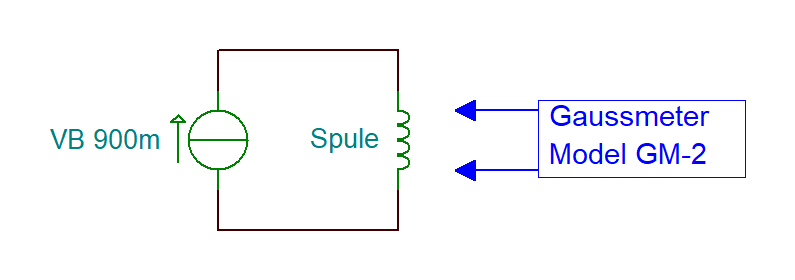
\includegraphics[scale=0.35]{measure_circuit.png}
  \caption{Messschaltung}
  \label{fig:measure_circuit}
\end{figure}

Die Spule wird vertikal aufgestellt und die Messsonde wird von oben hineingehalten. Hier sollte bemerkt werden, dass die Sonde des Gaussmeters immer in Richtung der gemessenen Feldlinien zeigt. Das Messgerät wird in der Mitte der Spule genullt (\textit{relative zero}).

\begin{figure}[h]
  \centering
  \input{assets/pipe_meas_sonde.pdf_tex}
  \caption{Sonde }
  \label{fig:measure_direction}
\end{figure}

Für die Widerstandsmessung wird mit dem Multimeter der Virtual Bench die Spule und die Messkabel selbst gemessen. Da beide Widerstände in Serie verbunden sind, kann der Kabelwiderstand vom Gesamtwiderstand abgezogen werden.

\begin{figure}[h]
  \centering
  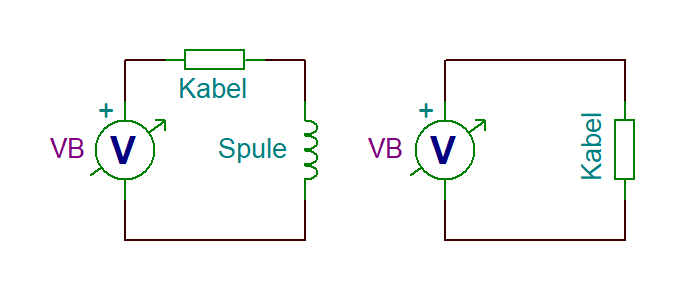
\includegraphics[scale=0.35]{assets/measure_resistance.PNG}
  \caption{Messschaltung für Widerstandsmessung}
  \label{fig:measure_resistance}
\end{figure}

\subsection{Messgeräte}

\begin{itemize}
  \item \textit{NI} Virtual Bench 'EL-13-041' (Multimeter \& Powersupply)
  \item \textit{AlphaLab Inc.} Gaussmeter Model GM-2
\end{itemize}

\end{document}
